% Options for packages loaded elsewhere
\PassOptionsToPackage{unicode}{hyperref}
\PassOptionsToPackage{hyphens}{url}
%
\documentclass[
]{article}
\usepackage{amsmath,amssymb}
\usepackage{iftex}
\ifPDFTeX
  \usepackage[T1]{fontenc}
  \usepackage[utf8]{inputenc}
  \usepackage{textcomp} % provide euro and other symbols
\else % if luatex or xetex
  \usepackage{unicode-math} % this also loads fontspec
  \defaultfontfeatures{Scale=MatchLowercase}
  \defaultfontfeatures[\rmfamily]{Ligatures=TeX,Scale=1}
\fi
\usepackage{lmodern}
\ifPDFTeX\else
  % xetex/luatex font selection
\fi
% Use upquote if available, for straight quotes in verbatim environments
\IfFileExists{upquote.sty}{\usepackage{upquote}}{}
\IfFileExists{microtype.sty}{% use microtype if available
  \usepackage[]{microtype}
  \UseMicrotypeSet[protrusion]{basicmath} % disable protrusion for tt fonts
}{}
\makeatletter
\@ifundefined{KOMAClassName}{% if non-KOMA class
  \IfFileExists{parskip.sty}{%
    \usepackage{parskip}
  }{% else
    \setlength{\parindent}{0pt}
    \setlength{\parskip}{6pt plus 2pt minus 1pt}}
}{% if KOMA class
  \KOMAoptions{parskip=half}}
\makeatother
\usepackage{xcolor}
\usepackage[margin=1in]{geometry}
\usepackage{graphicx}
\makeatletter
\def\maxwidth{\ifdim\Gin@nat@width>\linewidth\linewidth\else\Gin@nat@width\fi}
\def\maxheight{\ifdim\Gin@nat@height>\textheight\textheight\else\Gin@nat@height\fi}
\makeatother
% Scale images if necessary, so that they will not overflow the page
% margins by default, and it is still possible to overwrite the defaults
% using explicit options in \includegraphics[width, height, ...]{}
\setkeys{Gin}{width=\maxwidth,height=\maxheight,keepaspectratio}
% Set default figure placement to htbp
\makeatletter
\def\fps@figure{htbp}
\makeatother
\setlength{\emergencystretch}{3em} % prevent overfull lines
\providecommand{\tightlist}{%
  \setlength{\itemsep}{0pt}\setlength{\parskip}{0pt}}
\setcounter{secnumdepth}{-\maxdimen} % remove section numbering
\newlength{\cslhangindent}
\setlength{\cslhangindent}{1.5em}
\newlength{\csllabelwidth}
\setlength{\csllabelwidth}{3em}
\newlength{\cslentryspacingunit} % times entry-spacing
\setlength{\cslentryspacingunit}{\parskip}
\newenvironment{CSLReferences}[2] % #1 hanging-ident, #2 entry spacing
 {% don't indent paragraphs
  \setlength{\parindent}{0pt}
  % turn on hanging indent if param 1 is 1
  \ifodd #1
  \let\oldpar\par
  \def\par{\hangindent=\cslhangindent\oldpar}
  \fi
  % set entry spacing
  \setlength{\parskip}{#2\cslentryspacingunit}
 }%
 {}
\usepackage{calc}
\newcommand{\CSLBlock}[1]{#1\hfill\break}
\newcommand{\CSLLeftMargin}[1]{\parbox[t]{\csllabelwidth}{#1}}
\newcommand{\CSLRightInline}[1]{\parbox[t]{\linewidth - \csllabelwidth}{#1}\break}
\newcommand{\CSLIndent}[1]{\hspace{\cslhangindent}#1}
\usepackage{booktabs}
\usepackage{longtable}
\usepackage{array}
\usepackage{multirow}
\usepackage{wrapfig}
\usepackage{float}
\usepackage{colortbl}
\usepackage{pdflscape}
\usepackage{tabu}
\usepackage{threeparttable}
\usepackage{threeparttablex}
\usepackage[normalem]{ulem}
\usepackage{makecell}
\usepackage{xcolor}
\ifLuaTeX
  \usepackage{selnolig}  % disable illegal ligatures
\fi
\IfFileExists{bookmark.sty}{\usepackage{bookmark}}{\usepackage{hyperref}}
\IfFileExists{xurl.sty}{\usepackage{xurl}}{} % add URL line breaks if available
\urlstyle{same}
\hypersetup{
  pdftitle={Canadian Art Project Funding Ranges Prediction Using Random Forest},
  pdfauthor={Amelia Tang},
  hidelinks,
  pdfcreator={LaTeX via pandoc}}

\title{Canadian Art Project Funding Ranges Prediction Using Random
Forest}
\author{Amelia Tang}
\date{1/18/2022}

\begin{document}
\maketitle

{
\setcounter{tocdepth}{2}
\tableofcontents
}
\hypertarget{audiance-persona}{%
\section{Audiance Persona}\label{audiance-persona}}

Astrid is enrolled in a Data Science boot camp and is trying to switch
her career from freelance graphic design to data science. She has taken
basic math and statistics in college but might not be able to do math
proofs for machine learning algorithms. She has learned most of the
commonly used terminologies in data science, such as training/testing
data and different metrics. She also learned the general ideas of
popular machine learning algorithms from the boot camp. She is curious
about how machine learning can be applied to the real world. As a former
art practitioner, she is interested in how big data is used in the art
industry.

\hypertarget{abstract-executive-summary}{%
\section{Abstract / Executive
Summary}\label{abstract-executive-summary}}

The Government of Canada plays a vital role in preserving Canadian
heritage through funding art projects. Eligible Canadian artists and art
organizations may want to know the potential ranges of funding they can
receive for budgeting purposes. In this project, we built a predictive
model utilizing popular machine learning algorithms for multi-class
classifications, including Logistics Regression, Multinomial Naïve
Bayes, Support Vector Classification (SVC), and Random Forest. The model
predicted art projects' funding ranges using features such as the
projects' locations, disciplines, and target audiences, which were not
indicative of visual properties. We compared the performance of each
algorithm using three metrics: weighted average f-1, weighted-average
recall, and weighted-average precision. The results showed that the
random forest algorithm outperformed others with a weighted-average f-1
score of 0.69, a weighted-average recall of 0.69, and a weighted-average
precision of 0.69. Therefore, we could use the features non-indicative
of visual characteristics to predict the funding ranges that the
government would grant for art projects in Canada.

\hypertarget{introduction}{%
\section{Introduction}\label{introduction}}

The Canadian Arts Presentation Fund (``the Fund'') provides financial
assistance to arts festivals presenters and performing artists (Canada,
n.d.). The Fund's performance was evaluated based on the diversity of
the art projects it covered and broadness of the communities it reached.
The key mission of the Fund was to support a variety of art projects in
all parts of the country based on economic values that the projects
could bring to local communities ({``Grouped Arts Evaluation: Canada
Arts Presentation Fund, Canada Cultural Spaces Fund, and Canada Cultural
Investment Fund 2013-14 to 2017-18\_2019''} 2019).

In recent years, many studies used neural network algorithms and
features indicative of visual properties to predict values of art work.
However, the models with visual features, such as the image of the art
work, did not outperform the models using numeric and textual data only
(Aubry et al. 2022). In most cases, image data presenting the art work
alone failed to appraise the values (Ayub, Orban, and Mukund 2017).

In this project, we built classification models to predict approved
funding ranges of Canadian art projects based on textual features that
reflected social, cultural and geographical diversities. We did not add
any features related to the visual characteristics of the art projects.
After comparing the performances of four algorithms for multi-class
classification, logistics regression, Naïve Bayes, Support Vector
Classification (SVC) and Random Forest, we constructed a final
predictive model using Random Forest.

\hypertarget{methods}{%
\section{Methods}\label{methods}}

\hypertarget{data-collection}{%
\subsection{Data Collection}\label{data-collection}}

From fiscal year 2016-2017 and fiscal year 2017-2018, the Government of
Canada collected data on the art projects accepted and the funding sizes
approved. The data set is available on the Canada's Open Data website
and can be found
\href{https://open.canada.ca/data/en/dataset/92984c11-6fd4-40c4-b23c-e8832e1f4cd5}{here}.
The data set has 1358 rows of data. Each raw of the data contains the
project's name, location information, including community, city, region
and province, presenter information, such as organization names,
disciplines and target audience. The Fund also reported the funding size
for each art project in the data set. All the features included in this
data set were categorical features.

\hypertarget{data-processing}{%
\subsection{Data Processing}\label{data-processing}}

We observed that the funding sizes reported were not continuous, so we
divided the funding size data into five ranges, less than 8 thousand
Canadian dollars (\texttt{less\ than\ \$8.0k}), from 8 to 12 thousand
Canadian dollars (\texttt{\$8.0k-12.0k}), from 12 to 23 thousand
Canadian dollars (\texttt{\$12.0k-23.0k}), from 23 to 50 Canadian
dollars (\texttt{\$23.0k-\$50.0k}), and greater than 50 thousand
Canadian dollars (\texttt{over\ \$50.0k}). We used 10\%, 25\%, 50\% and
75\% percentiles of the funding size data as the cutoffs for the ranges.

When selecting features for our classification model, we noticed the
similar patterns of the funding ranges for each discipline in both
fiscal years. Therefore, fiscal year would not be a meaningful predictor
for funding ranges and we discarded this feature. Figure 1 showed the
detailed distributions for both fiscal years.

\begin{figure}

{\centering 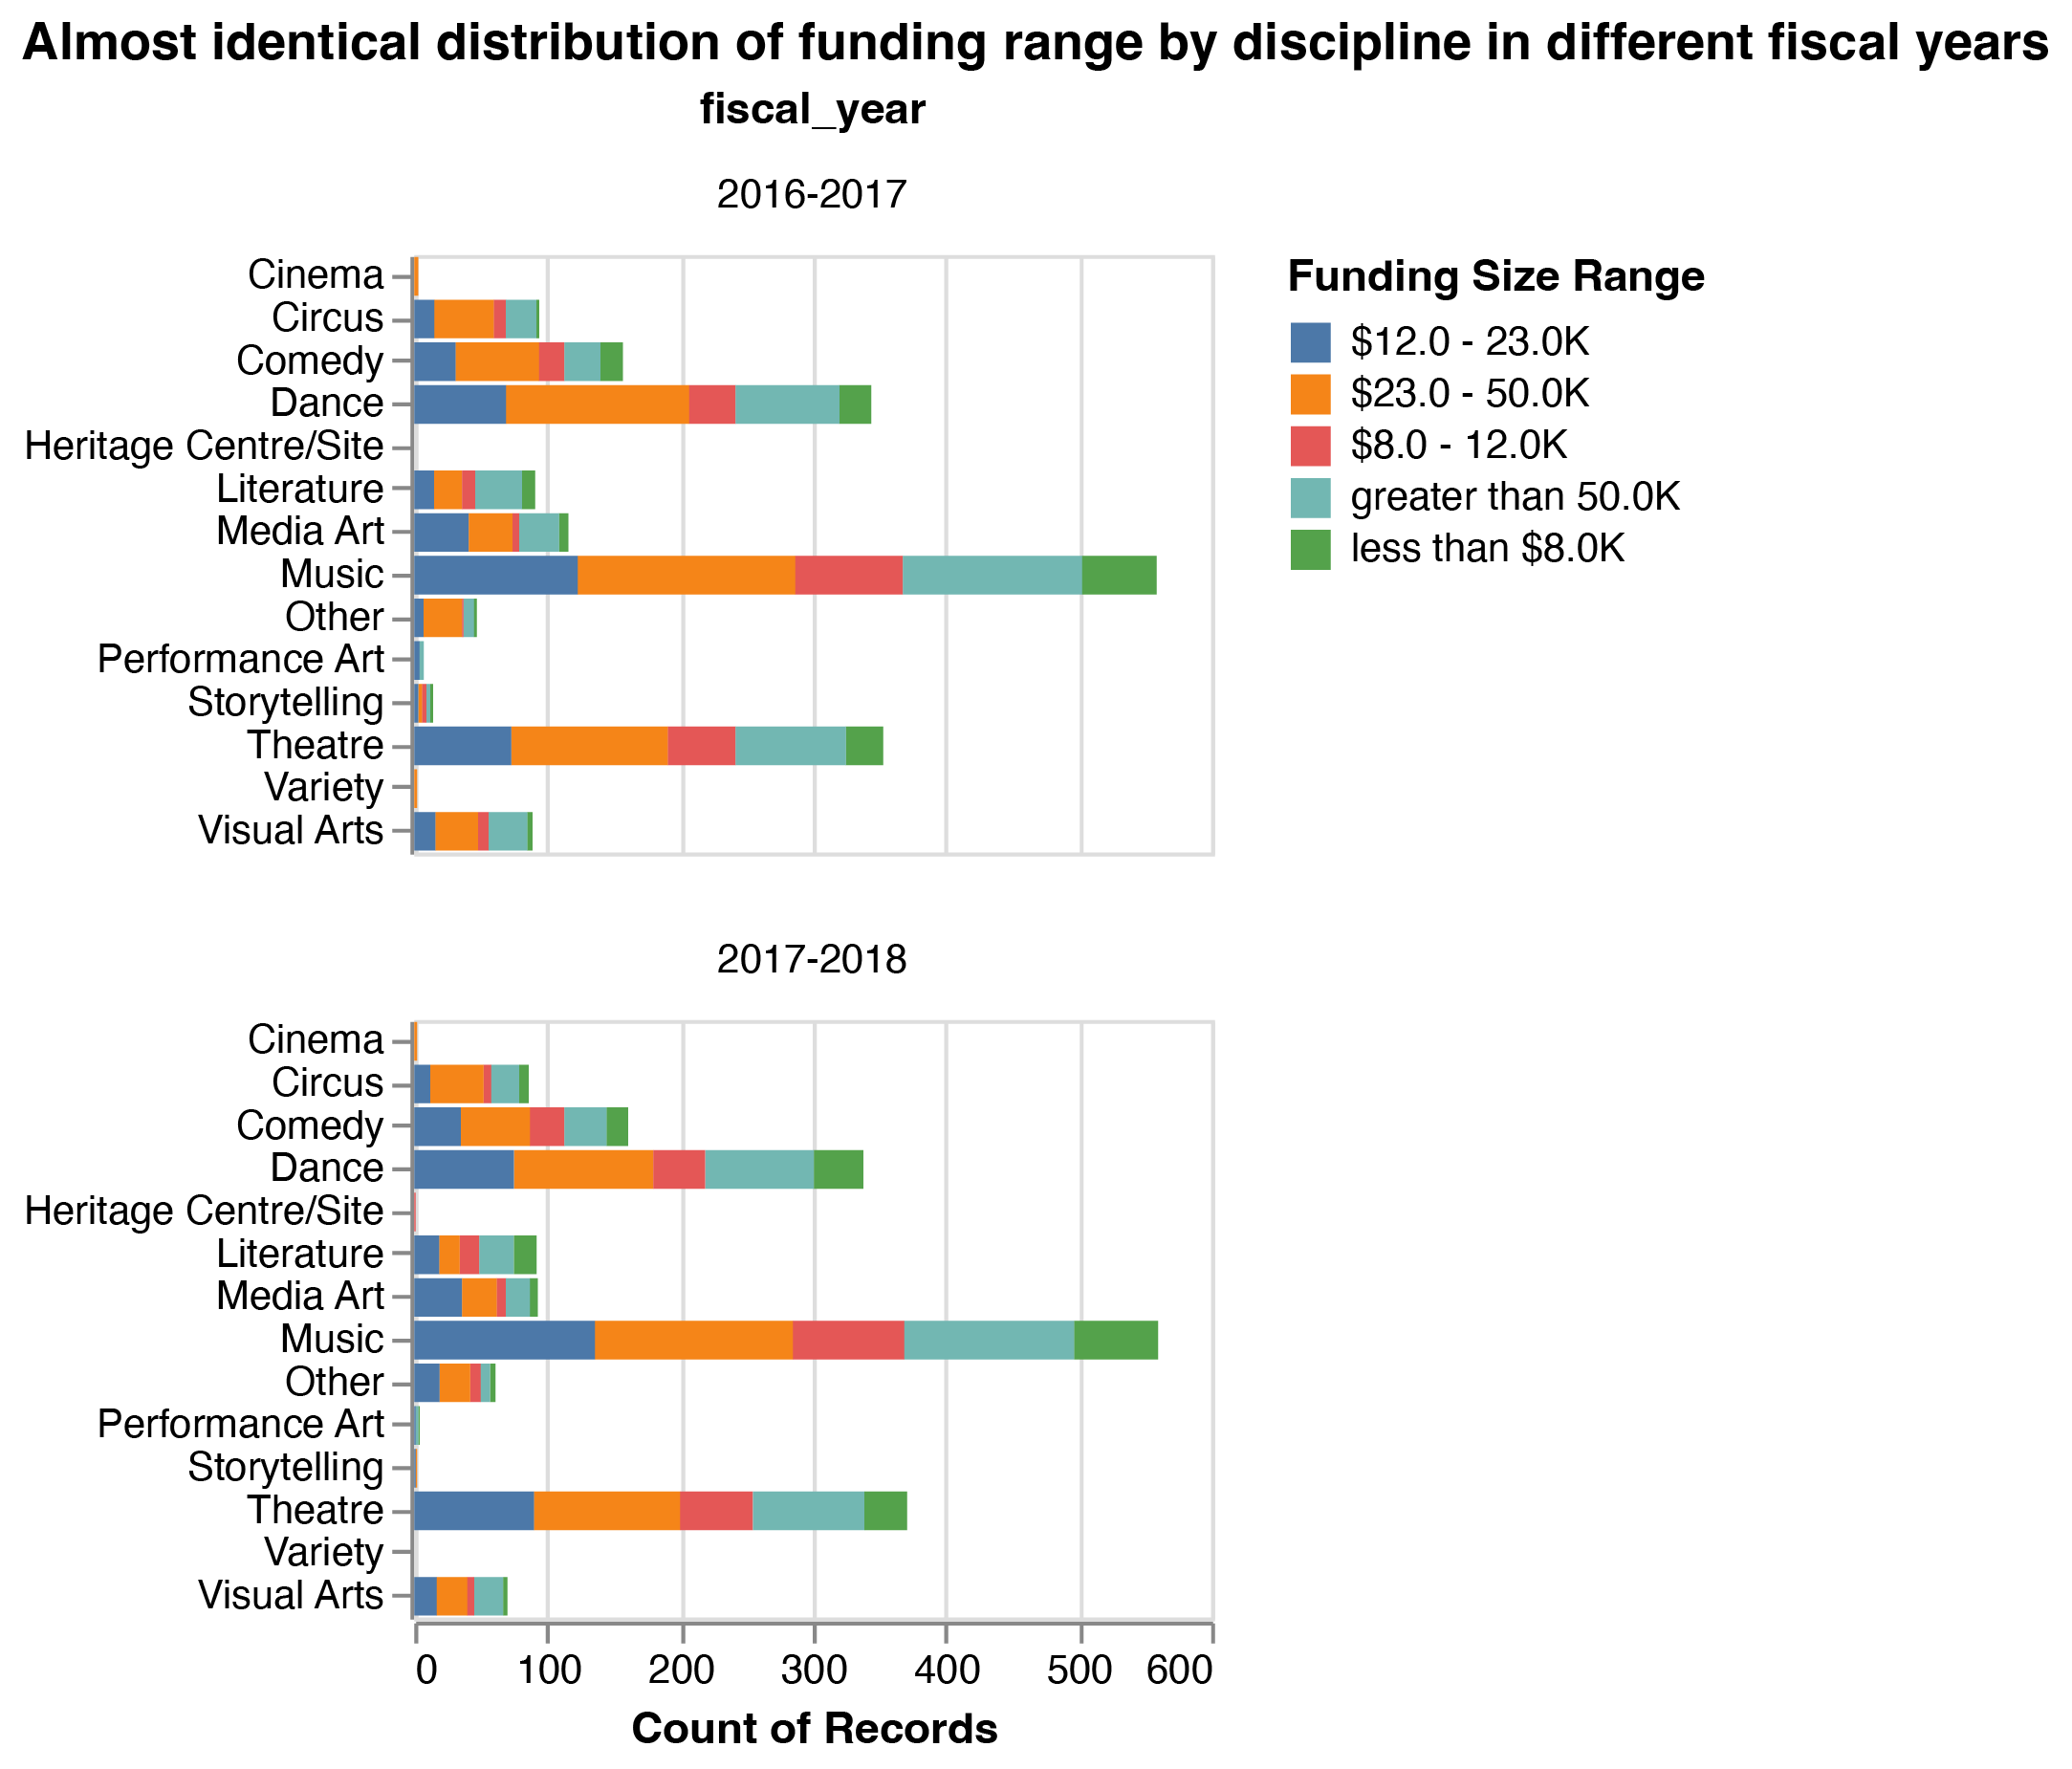
\includegraphics[width=0.7\linewidth]{../results/Funding_year} 

}

\caption{Comparison of the distribution of funding ranges 2016-2017 vs 2017-2018}\label{fig:drop-fiscal-year}
\end{figure}

We also discarded the data on regions because there was already data on
provinces of the art projects. It would be repetitive had we included
both. In addition, we excluded the organization names of the art
projects because there were too many unique names and thus would not be
informative when predicting funding ranges. Similarly, we did not choose
to use data on other disciplines because we already included data on
disciplines and there were many unique values in other disciplines. The
key features we included for our projects were province, community type,
grant or contribution, presenter type, project type, project sub-type,
disciplines and audiences.

\hypertarget{data-analysis}{%
\subsection{Data Analysis}\label{data-analysis}}

We used the Python programming language (Van Rossum and Drake 2009) and
the following Python packages to perform the analysis: numpy (Harris et
al. 2020), pandas (McKinney et al. 2010) and sikit-learn(Pedregosa et
al. 2011). The code used to perform the analysis and create this report
can be found
\href{https://github.com/UBC-MDS/canadian_heritage_funding}{here}.

We conducted a conventional 80:20 split to create the training and
testing data. We created a base-case model using the dummy classifier in
the scikit-learn package (Pedregosa et al. 2011) to serve as a
reference. Further, we chose four machine learning algorithms commonly
used for multi-class classification problems, Logistics Regression,
Multinomial Naïve Bayes, Support Vector Classification (SVC) and Random
Forest. We again used scikit-learn package (Pedregosa et al. 2011) to
build classification models.

There were class imbalances in our training dataset. Table 1 shows that
we had different sample sizes for the five ranges. To deal with this
issue, we set the class weight parameter to ``balanced'' for Logistics
Regression, Support Vector Classification (SVC), and Random Forest. When
set to balanced, the class weight parameter would tune the model to
assign a class weight inversely proportional to the sample size in each
class. We also set the max iteration parameter of Logistics Regression
to 1000 for the solver to converge.

\begin{table}[!h]

\caption{\label{tab:class_imbalance}Count of each funding ranges (Observed class imbalances)}
\centering
\begin{tabular}[t]{l|r}
\hline
Funding ranges & Count\\
\hline
over \$50.0K & 250\\
\hline
\$23.0-50.0K & 288\\
\hline
\$12.0-23.0K & 266\\
\hline
\$8.0-12.0K & 161\\
\hline
less than \$8.0K & 121\\
\hline
\end{tabular}
\end{table}

Because our problem was a multi-class classification problem, we used
relevant metrics, weighted-average f-1, weighted-average recall and
weighted-average precision to evaluate the model performances.

\hypertarget{results}{%
\section{Results}\label{results}}

After comparison, we found that the Random Forest model performed the
best among the four algorithms we used with our training dataset. We
also noticed that the Random Forest model required the longest fit time
for our data, though all four algorithms were reasonably time-efficient
and computationally inexpensive. Table 2 shows fit time,
weighted-average f-1, weighted-average recall, and weighted-average
precision for each model.

\begin{table}[!h]

\caption{\label{tab:model_compare}Random Forest performs the best}
\centering
\begin{tabular}[t]{l|r|r|r|r|r}
\hline
 & Dummy Classifier & Logistic Regression & Multinomial Naive Bayes & SVC & Random Forest\\
\hline
fit time & 0.03 & 0.31 & 0.03 & 0.19 & 0.43\\
\hline
score time & 0.02 & 0.02 & 0.02 & 0.04 & 0.04\\
\hline
weighted f1 & 0.11 & 0.57 & 0.44 & 0.52 & 0.63\\
\hline
weighted recall & 0.27 & 0.57 & 0.45 & 0.52 & 0.63\\
\hline
weighted precision & 0.07 & 0.58 & 0.47 & 0.53 & 0.64\\
\hline
\end{tabular}
\end{table}

To further tune the Random Forest model, we conducted hyperparameter
optimization and optimized the maximum number of features, class weight
(balanced or none), and maximum number of depths. The maximum number of
depths was important for tree-based models like Random Forest to avoid
overfitting.

Our tuned classification model using the Random Forest algorithm had a
weighted-average f-1 score of 0.69, a weighted-average recall of 0.69,
and a weighted-average precision of 0.69 when tested using our test
data. Table 3 shows the f-1 score, recall, and precision for each class.
The test scores were not the most ideal, but the model performed
reasonably well compared to the base-line model as well as the other
algorithms that we explored.

\begin{table}[!h]

\caption{\label{tab:best_model}Test Scores of the Tuned Random Forest Model}
\centering
\begin{tabular}[t]{l|r|r|r}
\hline
 & precision & recall & f1-score\\
\hline
less than \$8.0K & 0.79 & 0.70 & 0.74\\
\hline
\$8.0-12.0K & 0.74 & 0.68 & 0.71\\
\hline
\$12.0-23.0K & 0.61 & 0.60 & 0.60\\
\hline
\$23.0-50.0K & 0.58 & 0.63 & 0.61\\
\hline
over \$50.0K & 0.81 & 0.83 & 0.82\\
\hline
weighted average & 0.69 & 0.69 & 0.69\\
\hline
\end{tabular}
\end{table}

\hypertarget{conclusion}{%
\section{Conclusion}\label{conclusion}}

We provided a machine learning model to predict the funding ranges of
Canadian art projects using the Random Forest algorithm. This model
achieved some improvements over our base-case dummy classifier and other
algorithms that we explored: logistics regression, Multinomial Naïve
Bayes, and Support Vector Classification (SVC). We also found that
categorical features that described the basics of the art project, such
as location and presenter type, but did not contain information on the
visual properties, could reasonably predict the funding ranges approved
by the Canadian Arts Presentation Fund.

However, our model was not without limitations. We could further explore
techniques to solve the class imbalance problem for the Multinomial
Naïve Bayes algorithm. We might improve the model performance by
adjusting the cutoffs for the ranges to create more balanced classes. We
could expand our choices by exploring other algorithms such as k-Nearest
Neighbors. Moreover, we could add some features that were indicative of
visual properties of the art projects, such as the images of the
costumes, to see if the model would perform better.

\hypertarget{references}{%
\section*{References}\label{references}}
\addcontentsline{toc}{section}{References}

\hypertarget{refs}{}
\begin{CSLReferences}{1}{0}
\leavevmode\vadjust pre{\hypertarget{ref-aubry}{}}%
Aubry, Mathieu, Roman Kräussl, Gustavo Manso, and Christophe Spaenjers.
2022. {``Biased Auctioneers.''} \emph{SSRN}. Journal of Finance.
\url{https://papers.ssrn.com/sol3/papers.cfm?abstract_id=3347175\#}.

\leavevmode\vadjust pre{\hypertarget{ref-ayub}{}}%
Ayub, Rafi, Cedric Orban, and Vidush Mukund. 2017. {``Art Appraisal
Using Convolutional Neural Networks.''} \emph{CS229: Machine Learning}.
Stanford University.
\url{http://cs229.stanford.edu/proj2017/final-reports/5229686.pdf}.

\leavevmode\vadjust pre{\hypertarget{ref-canada}{}}%
Canada. n.d. \emph{Canada Arts Presentation Fund}. The Government of
Canada.
\url{https://www.canada.ca/en/canadian-heritage/services/funding/arts-presentation-fund.html}.

\leavevmode\vadjust pre{\hypertarget{ref-CandanaEvaServices}{}}%
{``Grouped Arts Evaluation: Canada Arts Presentation Fund, Canada
Cultural Spaces Fund, and Canada Cultural Investment Fund 2013-14 to
2017-18\_2019.''} 2019. The Government of Canada.
\url{https://www.canada.ca/en/canadian-heritage/corporate/publications/evaluations/grouped-art-evaluation.html\#a1}.

\leavevmode\vadjust pre{\hypertarget{ref-2020NumPy-Array}{}}%
Harris, Charles R., K. Jarrod Millman, Stéfan J van der Walt, Ralf
Gommers, Pauli Virtanen, David Cournapeau, Eric Wieser, et al. 2020.
{``Array Programming with {NumPy}.''} \emph{Nature} 585: 357--62.
\url{https://doi.org/10.1038/s41586-020-2649-2}.

\leavevmode\vadjust pre{\hypertarget{ref-mckinney2010data}{}}%
McKinney, Wes et al. 2010. {``Data Structures for Statistical Computing
in Python.''} In \emph{Proceedings of the 9th Python in Science
Conference}, 445:51--56. Austin, TX.

\leavevmode\vadjust pre{\hypertarget{ref-pedregosa2011scikit}{}}%
Pedregosa, Fabian, Gaël Varoquaux, Alexandre Gramfort, Vincent Michel,
Bertrand Thirion, Olivier Grisel, Mathieu Blondel, et al. 2011.
{``Scikit-Learn: Machine Learning in Python.''} \emph{Journal of Machine
Learning Research} 12 (Oct): 2825--30.

\leavevmode\vadjust pre{\hypertarget{ref-Python}{}}%
Van Rossum, Guido, and Fred L. Drake. 2009. \emph{Python 3 Reference
Manual}. Scotts Valley, CA: CreateSpace.

\end{CSLReferences}

\end{document}
